\PassOptionsToPackage{dvipsnames}{xcolor}
\documentclass[aspectratio=169,11pt]{beamer}

% ===== CONFIGURATION ==================================================
\newcommand{\projecttitle}{Pricing Baku Homes from Scratch}
\newcommand{\projectsub}{A NumPy Decision Tree and Pegasos SVM on bina.az Listings}
\newcommand{\memberone}{Farhad Budagov}
\newcommand{\membertwo}{Murad Atlukhanov}
\newcommand{\memberthree}{Panah Guluyev}
\newcommand{\memberfour}{Mikayil Hasanov}
\newcommand{\repolink}{github.com/pnah6699-maker/bina-az}
\newcommand{\presdate}{18 October 2026}

\newcommand{\coursecode}{MLE-AI-201}
\newcommand{\coursename}{Machine Learning}
\newcommand{\institution}{AI Academy, National AI Center}
\newcommand{\semester}{Fall 2026}

% ===== PACKAGES ======================================================
\usepackage[T1]{fontenc}
\usepackage[utf8]{inputenc}
\usepackage{xcolor}
\usepackage{tabularx}
\usepackage{booktabs}
\usepackage{listings}
\usepackage{graphicx}
\usepackage{tikz}
\usetikzlibrary{shapes.geometric,arrows.meta,positioning,fit,backgrounds}
\graphicspath{{../report/figures/}}
% Azerbaijani schwa (ə) is not in the standard fonts: draw it as a rotated "e".
\DeclareUnicodeCharacter{0259}{\raisebox{1ex}{\rotatebox{180}{e}}}

% ===== BEAMER THEME (same look as the course template) ===============
\usetheme{default}
\usefonttheme{professionalfonts}
\setbeamertemplate{navigation symbols}{}

\definecolor{accent}{HTML}{0B3D91}
\definecolor{accent2}{HTML}{8B0000}
\definecolor{soft}{HTML}{F2F4F8}
\definecolor{ok}{HTML}{166534}

\setbeamercolor{title}{fg=accent}
\setbeamercolor{frametitle}{fg=accent}
\setbeamercolor{itemize item}{fg=accent}
\setbeamercolor{itemize subitem}{fg=accent}
\setbeamercolor{enumerate item}{fg=accent}
\setbeamercolor{block title}{bg=accent,fg=white}
\setbeamercolor{block body}{bg=soft,fg=black}
\setbeamercolor{block title alerted}{bg=accent2,fg=white}
\setbeamercolor{block body alerted}{bg=soft,fg=black}

\setbeamerfont{title}{size=\Large,series=\bfseries}
\setbeamerfont{frametitle}{size=\large,series=\bfseries}
\setbeamerfont{footline}{size=\tiny}

% Footer: project + course + slide number
\setbeamertemplate{footline}{%
  \leavevmode%
  \hbox to \paperwidth{\hspace*{2ex}\tiny\textit{\projecttitle}\hfill%
  \tiny\textit{\coursecode{} -- \semester{}}\hfill%
  \tiny\insertframenumber/\inserttotalframenumber\hspace*{2ex}}%
  \vskip1pt%
}

% ===== CODE LISTINGS =================================================
\definecolor{codegreen}{rgb}{0,0.55,0}
\definecolor{codepurple}{rgb}{0.55,0,0.78}
\lstdefinestyle{python}{
  language=Python,
  backgroundcolor=\color{soft},
  commentstyle=\color{codegreen},
  keywordstyle=\color{accent},
  stringstyle=\color{codepurple},
  basicstyle=\ttfamily\scriptsize,
  breaklines=true,
  frame=single,
  framerule=0.4pt,
  rulecolor=\color{black!30},
  columns=fullflexible,
  keepspaces=true,
}

% =====================================================================
\begin{document}

% ========== SLIDE 1: TITLE ===========================================
{%
\setbeamertemplate{footline}{}
\begin{frame}[plain]
  \begin{center}
    \vspace{0.4cm}
    {\small \textsc{\institution}}\\[0.2em]
    {\small \textsc{\coursecode{} -- \coursename{} -- \semester{}}}\\[1.0em]
    \rule{0.8\textwidth}{0.6pt}\\[0.4em]
    {\LARGE\bfseries\color{accent} \projecttitle}\\[0.3em]
    {\large\color{accent} \projectsub}\\[0.3em]
    \rule{0.8\textwidth}{0.6pt}\\[1.0em]
    {\normalsize \memberone\quad\textbullet\quad\membertwo\quad\textbullet\quad\memberthree\quad\textbullet\quad\memberfour}\\[0.9cm]
    {\footnotesize\itshape Final Project Defense -- \presdate}\\[0.4em]
    {\footnotesize\texttt{\repolink}}
  \end{center}
\end{frame}
}

% ========== SLIDE 2: PROBLEM =========================================
\begin{frame}{The problem in one sentence}
  \begin{block}{What we built}
    Given a bina.az sale listing (size, rooms, floor, location, condition),
    predict its \textbf{price} and whether it is a \textbf{premium} or
    \textbf{standard} home --- with a decision tree and an SVM that we wrote
    \emph{from scratch in NumPy}, benchmarked honestly against scikit-learn.
  \end{block}

  \vspace{0.3em}
  \begin{columns}[T,onlytextwidth]
  \column{0.48\textwidth}
  \textbf{Task A --- Regression}
  \begin{itemize}
    \item Target: $\log(\text{price})$ (price skew 5.5 $\rightarrow$ 0.29)
    \item Model: our decision tree (MSE)
    \item Metrics: RMSE, MAE, $R^2$, MAPE
  \end{itemize}

  \column{0.48\textwidth}
  \textbf{Task B --- Classification}
  \begin{itemize}
    \item Premium $=$ price $>$ \textbf{train} median (209{,}000 AZN)
    \item Models: our tree (Gini/entropy), Pegasos SVM, RFF-SVM
    \item Metrics: precision, recall, F1, ROC-AUC
  \end{itemize}
  \end{columns}

  \vspace{0.4em}
  \textbf{One command reproduces everything:} \texttt{python -m src.run\_all}
\end{frame}

% ========== SLIDE 3: DATA FROM KAGGLE ================================
\begin{frame}[fragile]{Getting the data from Kaggle}
  \begin{columns}[T,onlytextwidth]
  \column{0.52\textwidth}
  \textbf{Source}
  \begin{itemize}\setlength\itemsep{0.2em}
    \item Kaggle: \texttt{sehriyarmemmedli/}\\\texttt{binaaz-sale-project} (version 1)
    \item \texttt{house\_sale.csv}: \textbf{100{,}775 rows $\times$ 51 columns}, 142\,MB
    \item Scraped from bina.az, 5--16 October 2024, all prices in AZN
    \item Azerbaijani column names: \textit{Sahə, Otaq sayı, Mərtəbə, Təmir} \ldots
  \end{itemize}

  \vspace{0.3em}
  \textbf{Not committed to Git} (\texttt{data/} is in \texttt{.gitignore});
  every member downloads it locally.

  \column{0.45\textwidth}
  \textbf{How we download it} (no API key needed)
\begin{lstlisting}[style=python]
# scripts/download_data.py
import kagglehub, shutil
path = kagglehub.dataset_download(
  "sehriyarmemmedli/binaaz-sale-project")
shutil.copyfile(path + "/house_sale.csv",
                "data/house_sale.csv")
\end{lstlisting}
\begin{lstlisting}[style=python,language=bash]
$ python scripts/download_data.py
\end{lstlisting}
  \end{columns}
\end{frame}

% ========== SLIDE 4: CLEANING & LEAKAGE ==============================
\begin{frame}{Cleaning a messy scrape --- and removing leakage}
  \begin{columns}[T,onlytextwidth]
  \column{0.50\textwidth}
  \textbf{Cleaning funnel}\\[0.2em]
  {\scriptsize
  \begin{tabular}{@{}lr@{}}
    \toprule
    Step & Rows \\
    \midrule
    Raw dump & 100{,}775 \\
    Keep latest scrape per listing URL & 64{,}454 \\
    Residential only (new / old / house) & 58{,}452 \\
    Drop exact re-posts & 57{,}699 \\
    Price 10k--5M AZN, area 15--1000\,m$^2$ & 57{,}594 \\
    Price/m$^2$ sanity, coords in AZ & \textbf{57{,}473} \\
    \bottomrule
  \end{tabular}}

  \vspace{0.3em}
  {\footnotesize Parsed \texttt{"145 m²"}, \texttt{"4.5 sot"}, \texttt{"7 / 9"};
  median imputation + missing flags $\rightarrow$ \textbf{92 features}.}

  \column{0.46\textwidth}
  \begin{alertblock}{Leakage removed}
    \begin{itemize}
      \item \texttt{unit\_price} = price / area
      \item \texttt{total\_price} = price
      \item IDs, owner names, address, \texttt{views}
    \end{itemize}
  \end{alertblock}
  \begin{block}{No test-set peeking}
    Featurizer, tier threshold and scaler are fit on \textbf{train only}
    (and re-fit inside every CV fold). Split 70/15/15, stratified.
  \end{block}
  \end{columns}
\end{frame}

% ========== SLIDE 5: EDA =============================================
\begin{frame}{What the data looks like}
  \begin{center}
    \includegraphics[height=0.36\textheight]{eda_price_distribution.pdf}\hfill
    \includegraphics[height=0.36\textheight]{eda_location.pdf}\\[0.1em]
    \includegraphics[height=0.33\textheight]{eda_area_vs_price.pdf}\hfill
    \includegraphics[height=0.33\textheight]{eda_rooms.pdf}\hfill
    \includegraphics[height=0.33\textheight]{eda_district.pdf}
  \end{center}
\end{frame}

% ========== SLIDE 6: PIPELINE ========================================
\begin{frame}{Pipeline: one command, every number}
  \begin{center}
  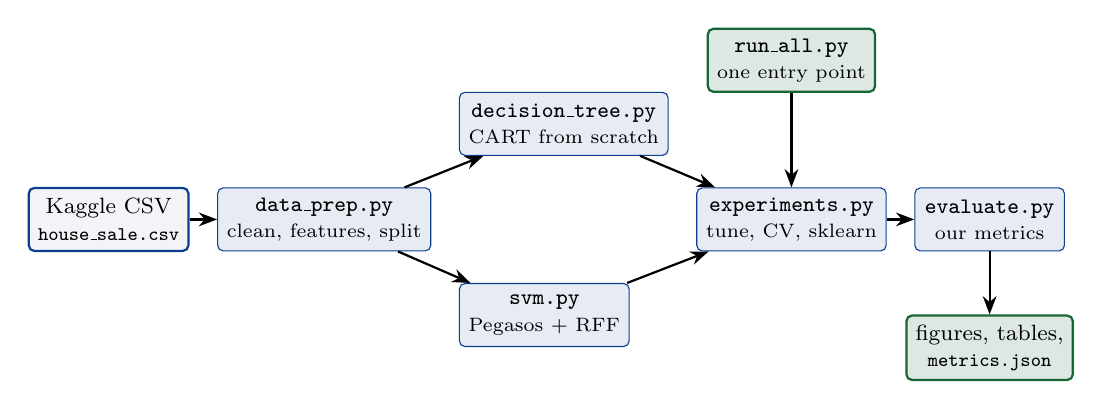
\begin{tikzpicture}[
    node distance=4mm and 3.5mm,
    box/.style={draw,rounded corners=2pt,minimum width=1.9cm,minimum height=0.8cm,align=center,font=\footnotesize},
    data/.style={box,fill=soft,draw=accent,thick},
    ours/.style={box,fill=accent!10,draw=accent},
    outbox/.style={box,fill=ok!15,draw=ok,thick},
    arrow/.style={-Stealth,thick}
  ]
    \node[data] (csv) {Kaggle CSV\\\scriptsize\texttt{house\_sale.csv}};
    \node[ours,right=of csv] (prep) {\texttt{data\_prep.py}\\\scriptsize clean, features, split};
    \node[ours,above right=of prep] (tree) {\texttt{decision\_tree.py}\\\scriptsize CART from scratch};
    \node[ours,below right=of prep] (svm) {\texttt{svm.py}\\\scriptsize Pegasos + RFF};
    \node[ours,below right=of tree] (exp) {\texttt{experiments.py}\\\scriptsize tune, CV, sklearn};
    \node[ours,right=of exp] (eval) {\texttt{evaluate.py}\\\scriptsize our metrics};
    \node[outbox,below=8mm of eval] (res) {figures, tables,\\\scriptsize\texttt{metrics.json}};
    \node[outbox,above=12mm of exp] (run) {\texttt{run\_all.py}\\\scriptsize one entry point};

    \draw[arrow] (csv) -- (prep);
    \draw[arrow] (prep) -- (tree);
    \draw[arrow] (prep) -- (svm);
    \draw[arrow] (tree) -- (exp);
    \draw[arrow] (svm) -- (exp);
    \draw[arrow] (exp) -- (eval);
    \draw[arrow] (eval) -- (res);
    \draw[arrow] (run) -- (exp);
  \end{tikzpicture}
  \end{center}

  \vspace{0.2em}
  {\footnotesize Blue boxes = our code. scikit-learn appears \textbf{only} as a
  baseline inside \texttt{experiments.py} and in the tests. Full run: 11 minutes on a laptop CPU, seed 42.}
\end{frame}

% ========== SLIDE 7: DECISION TREE ===================================
\begin{frame}{Our decision tree (NumPy only)}
  \begin{columns}[T,onlytextwidth]
  \column{0.50\textwidth}
  \textbf{How it grows}
  \begin{itemize}\setlength\itemsep{0.25em}
    \item Impurity: Gini $1-\sum p_k^2$, entropy $-\sum p_k\log_2 p_k$, MSE
    \item Split = feature/threshold with the largest gain\\
      $IG = I(\text{parent}) - \sum_c \frac{N_c}{N} I(c)$
    \item Sort each feature \textbf{once}; score all cut points with cumulative sums
    \item Stops: \texttt{max\_depth}, \texttt{min\_samples\_split},
          \texttt{min\_samples\_leaf}, \texttt{min\_impurity\_decrease}
    \item Leaf = mean or class frequencies (\texttt{predict\_proba})
  \end{itemize}

  \column{0.46\textwidth}
  \begin{block}{Does it match scikit-learn?}
    \begin{itemize}
      \item Toy 8-row example: \textbf{identical} splits \& thresholds
      \item Real data: same depth, leaves $\pm$4, \textbf{94.5\% / 98.9\%} identical predictions
      \item Differences = \textbf{ties}: ours \texttt{area}$\le$100.1, sklearn \texttt{log\_area}$\le$4.606 --- same split, since $e^{4.606}=100.1$
    \end{itemize}
  \end{block}
  \end{columns}
\end{frame}

% ========== SLIDE 8: PEGASOS SVM =====================================
\begin{frame}[fragile]{Our SVM: Pegasos sub-gradient descent}
  \begin{columns}[T,onlytextwidth]
  \column{0.52\textwidth}
  $J(\mathbf w)=\frac{\lambda}{2}\lVert\mathbf w\rVert^2+\frac1n\sum_i\max(0,1-y_i\,\mathbf w^\top\mathbf x_i)$
\begin{lstlisting}[style=python,basicstyle=\ttfamily\tiny]
eta = 1.0 / (lam * t)          # step size
active = yb * (Xb @ wb) < 1.0  # wrong / in margin
grad = (yb[active, None] * Xb[active]).sum(0)/k
wb *= (1.0 - eta * lam)        # shrink: wider margin
wb += eta * grad               # fix the mistakes
\end{lstlisting}
  \begin{itemize}\setlength\itemsep{0.15em}
    \item Mini-batches of 32, 30 epochs, bias folded into $\mathbf w$
    \item $J$: 1.00 $\rightarrow$ 0.270 (1 epoch) $\rightarrow$ 0.256
  \end{itemize}

  \column{0.45\textwidth}
  \begin{block}{A margin you can see ($\lambda=0.01$)}
    $\lVert\mathbf w\rVert = 2.09$, margin $2/\lVert\mathbf w\rVert = 0.96$\\
    Support vectors: \textbf{11{,}135} (27.7\%)
  \end{block}
  \begin{block}{Non-linear: random Fourier features}
    $z(\mathbf x)=\sqrt{2/D}\cos(W\mathbf x+c)$, $D=1000$, then the same
    linear solver. Chosen over kernel Pegasos: $O(D)$ vs.\ $O(n)$ per step on 40k rows.
  \end{block}
  \end{columns}
\end{frame}

% ========== SLIDE 9: TUNING ==========================================
\begin{frame}{Tuning on validation only: bias vs.\ variance}
  \begin{center}
    \includegraphics[width=0.49\textwidth]{tree_regression_tuning.pdf}\hfill
    \includegraphics[width=0.49\textwidth]{tree_classification_tuning.pdf}\\[0.1em]
    \includegraphics[width=0.75\textwidth]{svm_lambda_sweep.pdf}
  \end{center}
  {\footnotesize Selected: tree A depth 17 / leaf 5; tree B Gini, depth 14; SVM $\lambda=0.01$ (larger $\lambda$ $\Rightarrow$ wider margin, more support vectors).}
\end{frame}

% ========== SLIDE 10: RESULTS ========================================
\begin{frame}{Results: test set (5-fold CV mean $\pm$ std)}
  \begin{center}\small
  \begin{tabular}{lccc}
    \toprule
    \textbf{Model} & \textbf{Task A RMSE (log)} & \textbf{Task B F1} & \textbf{ROC-AUC} \\
    \midrule
    \textbf{Ours: decision tree} & \textbf{0.232} (0.232$\pm$0.004) & \textbf{0.921} (0.926$\pm$0.004) & 0.917 \\
    sklearn DecisionTree         & 0.232 (0.233$\pm$0.004) & 0.921 (0.926$\pm$0.004) & 0.916 \\
    \midrule
    \textbf{Ours: Pegasos SVM}   & --- & \textbf{0.900} (0.907$\pm$0.003) & 0.965 \\
    sklearn SGD hinge            & --- & 0.900 (0.908$\pm$0.003) & 0.965 \\
    \textbf{Ours: RFF SVM}       & --- & 0.900 (0.906$\pm$0.003) & 0.967 \\
    \midrule
    Mean / majority baseline     & 0.629 & 0.000 & 0.500 \\
    \bottomrule
  \end{tabular}
  \end{center}

  \vspace{0.3em}
  \begin{itemize}\setlength\itemsep{0.2em}
    \item Task A: $R^2=0.864$, MAPE 15.4\%, MAE $\approx$ 44.6k AZN
    \item Ours = sklearn within \textbf{0.002} on every metric; ours is $\sim$10$\times$ slower (6.6\,s vs 0.5\,s)
    \item Tree wins F1, SVM wins AUC: leaf frequencies are coarse scores, the SVM ranks smoothly
  \end{itemize}
\end{frame}

% ========== SLIDE 11: ERROR ANALYSIS =================================
\begin{frame}{Where the models fail}
  \begin{columns}[T,onlytextwidth]
  \column{0.55\textwidth}
  \includegraphics[width=\linewidth]{error_by_price_decile.pdf}\\[0.2em]
  \includegraphics[width=0.49\linewidth]{error_by_location_frequency.pdf}\hfill
  \includegraphics[width=0.49\linewidth]{tier_error_vs_distance.pdf}

  \column{0.42\textwidth}
  \begin{itemize}\setlength\itemsep{0.35em}
    \item \textbf{Luxury \& bargain outliers:} cheapest decile over-predicted, most expensive under-predicted (MAPE 26\% / 22\% vs.\ 12\% mid)
    \item \textbf{Houses/villas:} 32\% MAPE vs.\ 12\% for flats
    \item \textbf{Sparse locations} ($<$150 train rows): 29.9\% vs.\ 14.3\% MAPE
    \item \textbf{Tier errors at the boundary:} 38--46\% wrong within 5\% of the median, $<$2\% beyond 50\%
    \item Worst cases: instalments listed as the price
  \end{itemize}
  \end{columns}
\end{frame}

% ========== SLIDE 12: BONUSES ========================================
\begin{frame}{Bonus work}
  \begin{columns}[T,onlytextwidth]
  \column{0.36\textwidth}
  \textbf{P8 --- Ridge (normal equations)}
  \begin{itemize}
    \item $\hat{\mathbf w}=(X^\top X+\lambda I)^{-1}X^\top\mathbf y$
    \item RMSE 0.242; coefficients $=$ sklearn to $10^{-10}$
  \end{itemize}
  \vspace{0.2em}
  \textbf{P9 --- Random forest of our trees}
  \begin{itemize}
    \item 30 trees, bootstrap + 33\% features
    \item RMSE \textbf{0.264 $\rightarrow$ 0.185}; sklearn: 0.185
  \end{itemize}

  \column{0.30\textwidth}
  \includegraphics[width=\linewidth]{bonus_random_forest.pdf}

  \column{0.30\textwidth}
  \textbf{P10 --- k-means \& PCA}
  \includegraphics[width=\linewidth,trim=0 0 0 0,clip]{bonus_clusters_pca.pdf}
  \end{columns}
\end{frame}

% ========== SLIDE 13: TESTING & REPRODUCIBILITY ======================
\begin{frame}[fragile]{Testing \& reproducibility}
  \begin{columns}[T,onlytextwidth]
  \column{0.52\textwidth}
  \textbf{40 unit tests, all passing} (\texttt{pytest})
  \begin{itemize}\setlength\itemsep{0.25em}
    \item Tree splits $=$ sklearn on a fully determined toy example
    \item Every stopping rule changes the tree
    \item SVM objective decreases; larger $\lambda$ $\Rightarrow$ wider margin
    \item RFF approximates the RBF kernel and solves XOR
    \item Our metrics $=$ \texttt{sklearn.metrics}; leakage columns dropped
  \end{itemize}

  \column{0.45\textwidth}
  \textbf{From a clean checkout}
\begin{lstlisting}[style=python,language=bash]
$ pip install -r requirements.txt
$ python scripts/download_data.py
$ python -m src.run_all
$ python -m pytest -q
\end{lstlisting}
  \begin{itemize}\setlength\itemsep{0.2em}
    \item Pinned versions, seed 42 everywhere
    \item Tables in the report are generated by code
  \end{itemize}
  \end{columns}
\end{frame}

% ========== SLIDE 14: LIMITATIONS + FUTURE ===========================
\begin{frame}{Limitations \& what we would improve}
  \textbf{Where the project is weak today}
  \begin{itemize}\setlength\itemsep{0.25em}
    \item \emph{Asking} prices from an 11-day snapshot --- not real transaction prices
    \item Fixed outlier rules miss some instalment prices and drop villas above 5M AZN
    \item Free-text descriptions (renovation, documents, view) are unused
    \item Our NumPy tree is $\sim$10$\times$ slower than compiled code $\Rightarrow$ less forest tuning
  \end{itemize}

  \vspace{0.3em}
  \textbf{Given another week we would}
  \begin{enumerate}\setlength\itemsep{0.25em}
    \item Add text features from the listing descriptions
    \item Use a time-based split, closer to real deployment
    \item Target-encode sparse micro-locations (biggest error source)
    \item Build gradient boosting from our own trees
  \end{enumerate}
\end{frame}

% ========== SLIDE 15: TEAM CONTRIBUTIONS =============================
\begin{frame}{Team contributions}
  \begin{center}\small
  \begin{tabularx}{\linewidth}{l>{\raggedright\arraybackslash}Xl}
    \toprule
    \textbf{Member} & \textbf{Primary ownership} & \textbf{Code share} \\
    \midrule
    \memberone   & Decision tree + metrics (\texttt{decision\_tree.py}, \texttt{evaluate.py}, tests) & 26\% \\
    \membertwo   & Data cleaning, features, EDA (\texttt{data\_prep.py}, \texttt{eda.py}, \texttt{plots.py}, tests) & 24\% \\
    \memberthree & Pegasos SVM + RFF, bonus models, pipeline (\texttt{svm.py}, \texttt{ensemble.py}, \texttt{linear.py}, \texttt{run\_all.py}) & 26\% \\
    \memberfour  & Experiments: tuning, sklearn benchmark, CV, error analysis (\texttt{experiments.py}) & 24\% \\
    \bottomrule
  \end{tabularx}
  \end{center}

  \vspace{0.3em}
  \begin{block}{We can all answer:}
    Any of us can walk through any module on demand. Pick a file --- we'll defend it.
  \end{block}

  \vspace{0.2em}
  \textbf{AI tool use:} Claude Code (Anthropic) drafted code, tests and report text;
  every member reviewed, ran and can explain their part (disclosed in the report).
\end{frame}

% ========== SLIDE 16: THANK YOU / Q&A ================================
{%
\setbeamertemplate{footline}{}
\begin{frame}[plain]
  \begin{center}
    \vspace{1cm}
    {\Huge\bfseries\color{accent} Questions?}\\[1.2em]
    \rule{0.5\textwidth}{0.6pt}\\[1.2em]
    {\normalsize \memberone\quad\textbullet\quad\membertwo\quad\textbullet\quad\memberthree\quad\textbullet\quad\memberfour}\\[0.6em]
    {\normalsize \texttt{\repolink}}\\[1cm]
    {\footnotesize\itshape ``We can walk through any file in the repo.''}
  \end{center}
\end{frame}
}

\end{document}
